\documentclass[a4j]{ujarticle}
\renewcommand{\baselinestretch}{0.85}
\usepackage[top=1.5cm, bottom=1.5cm, left=1.5cm, right=1.5cm]{geometry}
\usepackage{xcolor}
\usepackage[dvipdfmx]{graphicx, hyperref}
\usepackage{listings}
\usepackage{multirow}
\usepackage{siunitx}
\usepackage{subfig}
\usepackage{url}
\usepackage{caption,stackengine}

\newcommand{\Sref}[1]{\mbox{\ref{sec:#1}}}
\newcommand{\Tref}[1]{\mbox{表\ref{tab:#1}}}
\newcommand{\Eref}[1]{\mbox{式(\ref{eq:#1})}}
\newcommand{\Fref}[1]{\mbox{図\ref{fig:#1}}}
\renewcommand{\lstlistingname}{ソースコード}
\newcommand{\Lref}[1]{\mbox{ソースコード\ref{lst:#1}}}
\newcommand{\bhline}[1]{\noalign{\hrule height #1}}

\captionsetup[subfigure]{labelformat=simple}
\renewcommand{\thesubfigure}{(\alph{subfigure})}

\hypersetup{
	setpagesize=false,
	bookmarksnumbered=true,
	bookmarksopen=true,
	colorlinks=true,
	linkcolor=black,
	citecolor=black
}

\begin{document}
    \begin{flushright}
        MDLab GM資料\\
        22年10月18日(火)
    \end{flushright}

    \begin{center}
        {\Large	距離学習を導入したCenterNetによる\\腹部超音波画像からの肝腫瘍検出と分類}
    \end{center}

    \begin{flushright}
        {\large B4 原 英吾}\\
    \end{flushright}

    \section{研究背景および目的}
    \begin{figure}[h]
        \begin{minipage}{.59\textwidth}
            \begin{itemize}
                \item 背景
                \begin{itemize}
                    \item 器具の操作と診断を同時に行わなければならず高難易度
                    \item 機械学習による診断のサポート
                    \begin{itemize}
                        \item 良性・悪性を見分けることが重要視される
                        \item \Fref{ex}の様に明らかなラベル不足\footnotemark[1]のある画像が存在する
                    \end{itemize}
                    \item 先行研究では0.7617($\approx 0.8550 \times 0.8909$)
                    \begin{itemize}
                        \item 検出(Recall): 0.8550
                        \item 分類(Accuracy): 0.8909
                    \end{itemize}
                \end{itemize}
                \item 目的
                \begin{itemize}
                    \item 既存の研究を踏まえたモデルの精度向上
                    \item 超音波支援システムの開発
                \end{itemize}
            \end{itemize}
        \end{minipage}
        \begin{minipage}{.39\textwidth}
            \centering
            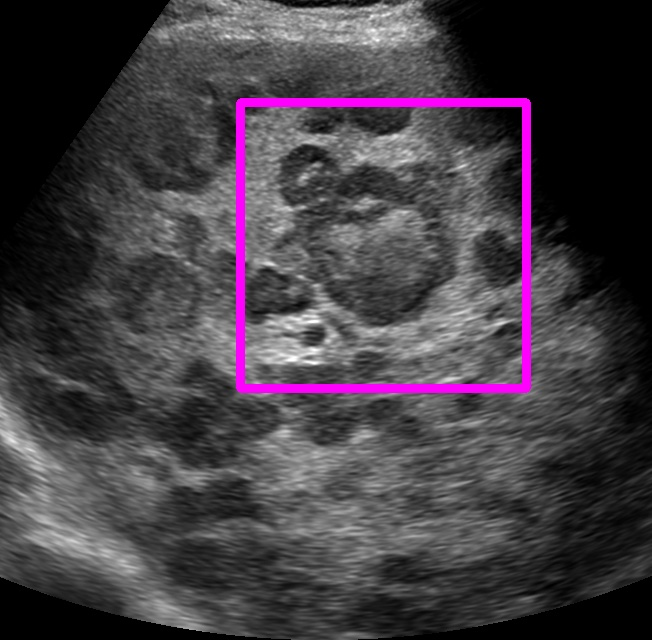
\includegraphics[width=.9\linewidth]{../fig/pseudo_a.png}
            \caption{ラベル不足のある診断画像例}
            \label{fig:ex}
        \end{minipage}
    \end{figure}

    \footnotetext[1]{今回は\Fref{ex}の様なアノテーションが不足しているものを指す}
    \addtocounter{footnote}{1}

    \section{これまでの研究のまとめ}
        \begin{itemize}
            \item データセット
            \begin{itemize}
                \item 国立研究開発法人日本医療研究開発機構(AMED)\footnote{\url{https://www.amed.go.jp/}}が提供している延べ8万枚に及ぶ以下のデータが付随
                \begin{itemize}
                    \item 腹部超音波画像,ROI
                    \item 年齢,性別
                \end{itemize}
                \begin{figure}[h]
                    \centering
                    \subfloat[性別毎の画像枚数]{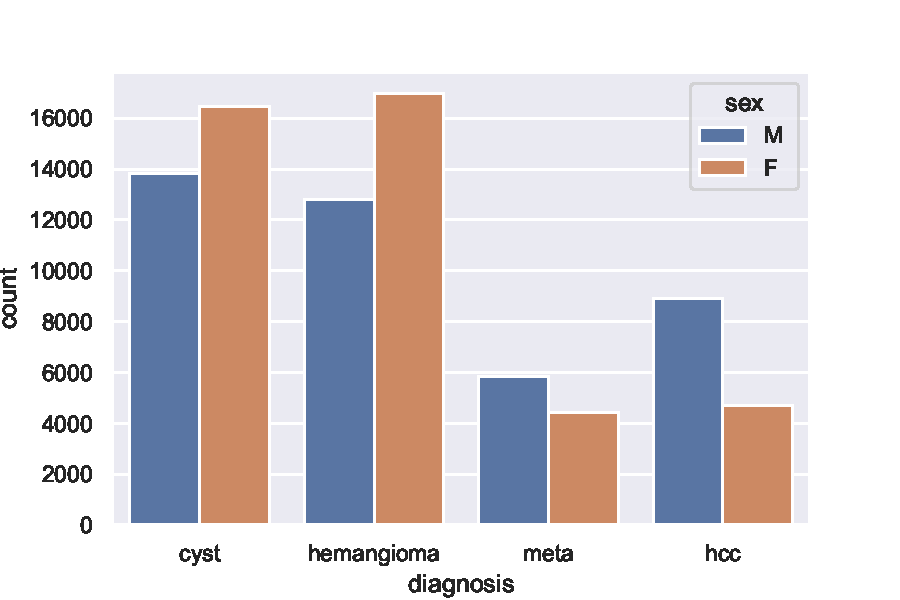
\includegraphics[width=.24\linewidth]{../fig/sex_a.pdf} \label{fig:sex}}
                    \subfloat[診断名毎の年齢分布]{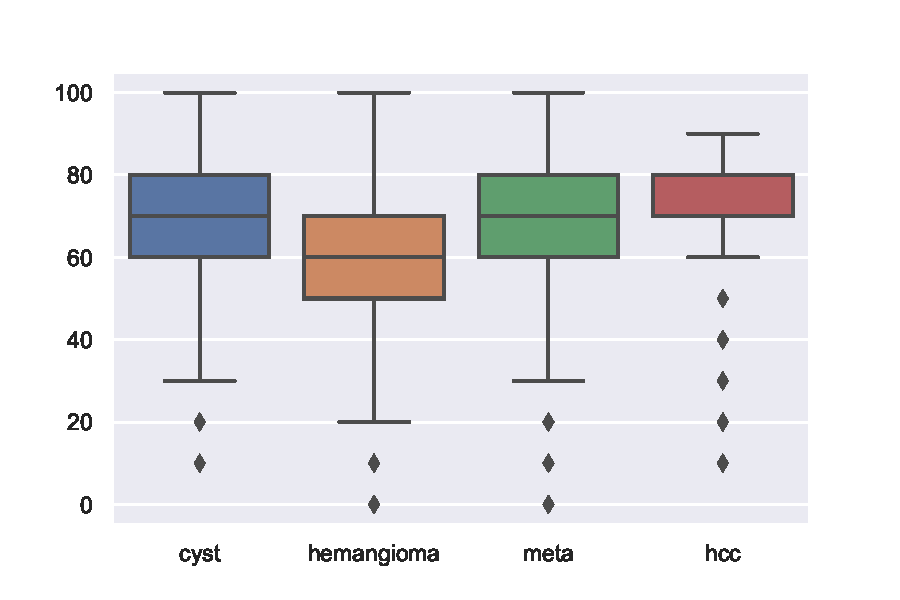
\includegraphics[width=.24\linewidth]{../fig/age_a.pdf} \label{fig:age}}
                    \subfloat[診断名毎の画像サイズの分布]{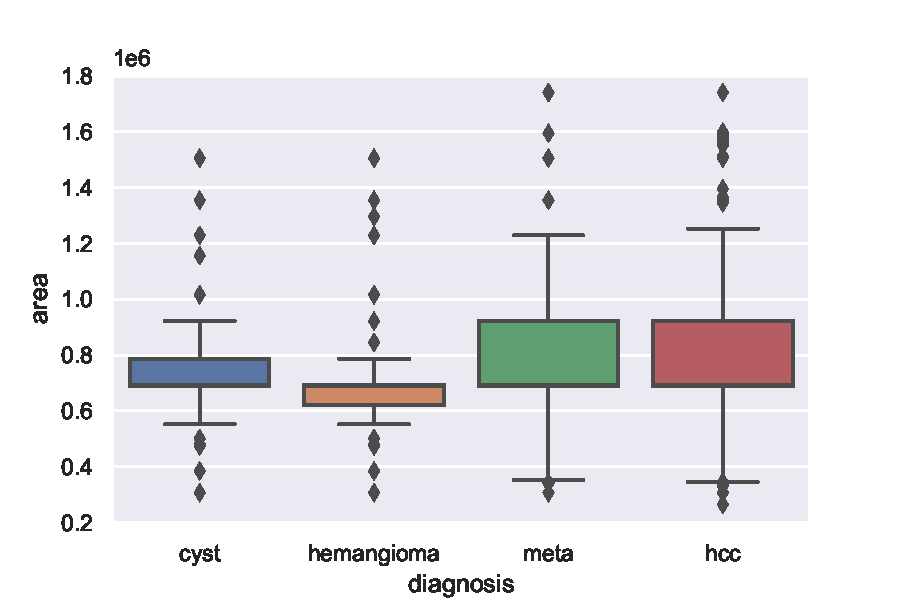
\includegraphics[width=.24\linewidth]{../fig/area_a.pdf} \label{fig:area}}
                    \subfloat[診断名毎のbboxの割合]{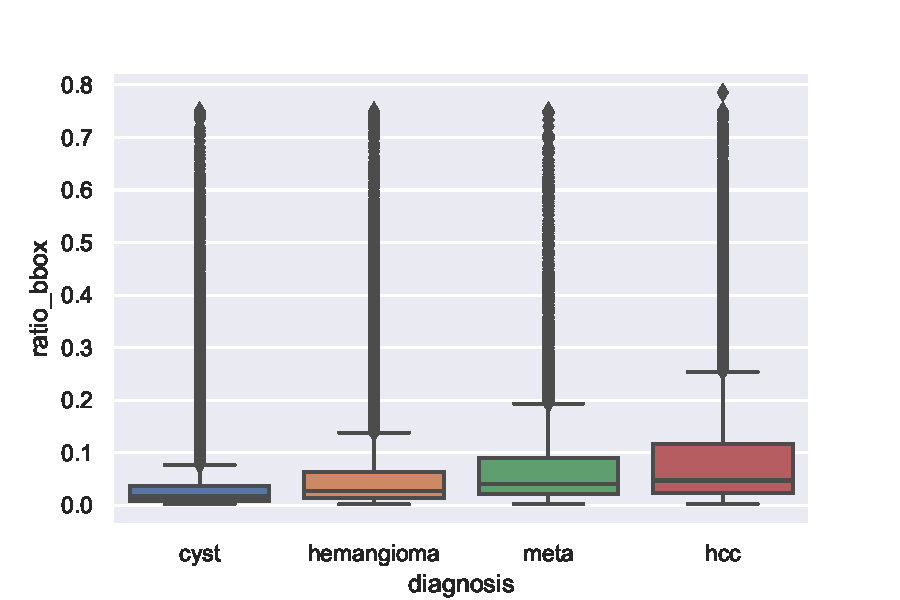
\includegraphics[width=.24\linewidth]{../fig/ratio_bbox_a.pdf} \label{fig:ratio}}
                    \caption{データセットにおけるデータの分布}
                \end{figure}
                \item 性別(\Fref{sex})
                \begin{itemize}
                    \item HCC(肝細胞癌)は男性が罹患しやすい
                    \begin{itemize}
                        \item 昔は男性の方が飲酒・タバコが多く癌に罹りやすかったという時代背景があるかもしれない
                    \end{itemize}
                    \item Hemangioma(血管腫)は女性が罹患しやすい
                    \item Meta(転移性肝癌)は他の症状よりも少ない
                \end{itemize}
                \item 年齢(\Fref{age})
                \begin{itemize}
                    \item Cyst(単純嚢胞),Hemangioma(血管腫)の分布にははあまり特徴がない
                    \item Hemangioma(血管腫)は比較的若年層でも罹患する
                    \item Meta(転移性肝癌)における0歳はラベルミスである可能性が高い
                    \item HCC(肝細胞癌)は比較的高齢者が罹患しやすい
                \end{itemize}
                \item 画像サイズ(\Fref{area})
                \begin{itemize}
                    \item Hemangioma(血管腫)は比較的画像サイズが統一されている
                    \begin{itemize}
                        \item 腫瘍の大きさが血管に依存するためあまり偏りが生じていない?
                    \end{itemize}
                \end{itemize}
                \item bboxの画像に占める割合(\Fref{ratio})
                \begin{itemize}
                    \item Cyst(単純嚢胞)は他の診断と比べてbboxの割合が低い($\frac{1}{2}$程度)である
                    \item HCC(肝細胞癌)は画像に占めるbboxの割合が高い
                \end{itemize}
            \end{itemize}
        \end{itemize}

        \begin{itemize}
            \item 症状毎の特徴を調査
            \begin{figure}[h]
                \centering
                \subfloat[Cyst(単純嚢胞)]{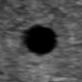
\includegraphics[width=.24\linewidth]{../fig/cyst.png} \label{fig:cyst}}
                \subfloat[HCC(肝細胞癌)]{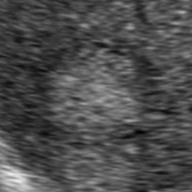
\includegraphics[width=.24\linewidth]{../fig/hcc.png} \label{fig:hcc}}
                \subfloat[hemangioma(血管腫)]{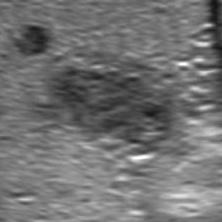
\includegraphics[width=.24\linewidth]{../fig/hemangioma.png} \label{fig:hemangioma}}
                \subfloat[Meta(転移性肝癌)]{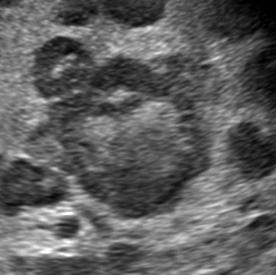
\includegraphics[width=.24\linewidth]{../fig/meta.png} \label{fig:meta}}
                \caption{症状毎における腫瘍の超音波画像}
            \end{figure}
            \begin{itemize}
                \item Cyst(単純嚢胞) (\Fref{cyst})
                \begin{itemize}
                    \item 液体が貯留されている状態の良性腫瘍
                    \item 症状がでないことが多いため大きな腫瘍になって発見されることが多い
                    \item 嚢胞の内腔に向けて増殖するため転移することは少ない
                \end{itemize}
                \item HCC(肝細胞癌) (\Fref{hcc})
                \begin{itemize}
                    \item 肝臓にできる\textcolor{red}{悪性腫瘍}の中で最も多いと言われている
                    \item 約90\%がウイルス感染症が原因
                    \begin{itemize}
                        \item B型肝炎ウイルス(HBV)が約20\%
                        \item C型肝炎ウイルス(HCV)が約70\%
                    \end{itemize}
                \end{itemize}
                \item Hemangioma(血管腫) (\Fref{hemangioma})
                \begin{itemize}
                    \item 肝臓にできる良性腫瘍の中で最も多い
                    \item 女性ホルモンが原因で女性が罹患しやすいと言われているが詳しくは解明されていない
                    \item 血管が無数に絡み合うことによって出来た血管の塊であることから血流が遅いという特徴がある
                    \item 他の臓器に浸潤したり転移することは無いと言われている
                \end{itemize}
                \item Meta(転移性肝癌) (\Fref{meta})
                \begin{itemize}
                    \item 門脈を介して大腸癌などの消化器癌から転移する割合が多い\textcolor{red}{悪性腫瘍}
                    \item 類似したエコーパターンをもつ腫瘤が多発してみられることが多い
                \end{itemize}
            \end{itemize}
        \end{itemize}

        \begin{itemize}
            \item データクレンジング
            \begin{enumerate}
                \item $400\times400$以下の画像の除外
                \item Perceptual Hashを利用した類似画像の除外
                \item 青色や黄色のスケールの除去
            \end{enumerate}

            \item 提供されているデータをCOCODatasetの形式に変換
            \begin{itemize}
                \item train data : test data : val data = 67122 : 8390 : 8391
                \item 見やすいようにインデントしたファイル\footnote{\url{//aka/work/hara.e/AMED/lib/dataset/annotations/train_large.json}など}も作成
            \end{itemize}
        \end{itemize}

\clearpage

    \section{前回のGMからの進捗}
        \begin{itemize}
            \item モデル・クラス数ごとの検出結果の比較

            \begin{figure}[!h]
                \centering
                \subfloat[1クラス検出時の混同行列]{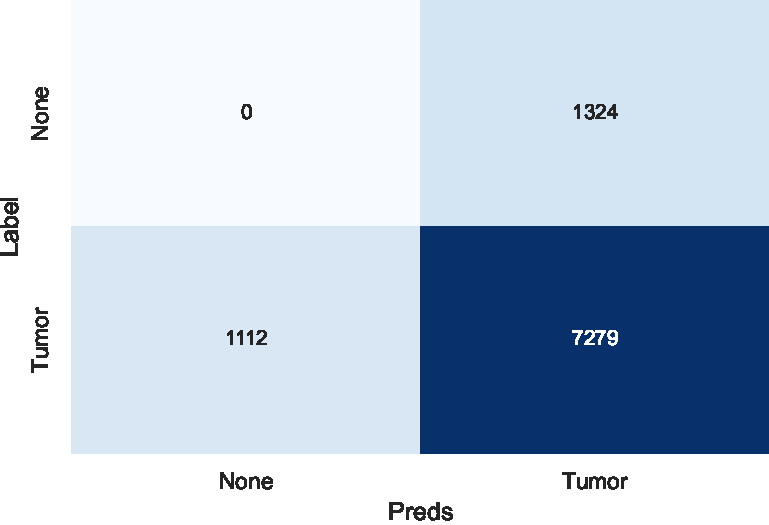
\includegraphics[width=.49\linewidth]{../fig/heatmap_centernet_tumor.pdf} \label{fig:cmat_tumor}}
                \subfloat[4クラス検出時の混同行列]{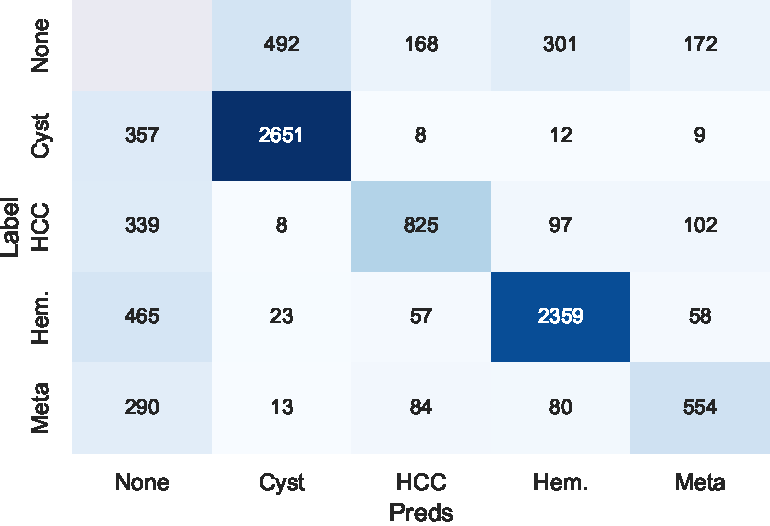
\includegraphics[width=.49\linewidth]{../fig/heatmap_centernet_stepwise2.pdf} \label{fig:cmat_step}}
                \caption{CenterNet\cite{centernet}で検出した時の混同行列}
            \end{figure}
        \end{itemize}

        \begin{table}[!h]
            \centering
            \caption{SimSiam\cite{simsiam}で距離学習後に段階的にbackboneの重みを解除したモデルでの評価指標毎の値}
            \label{tab:metric_center_stepwise}
            \begin{tabular}{c|ccc|ccc} \hline
                Diagnosis & データ総数 & FP & FN & precision & recall & f1-score \\ \hline
                Cyst & 3037 & 483 & 253 & 0.8405 & 0.9055 & 0.8718 \\
                HCC & 1371 & 112 & 363 & 0.7623 & 0.5872 & 0.6634 \\
                Hemangioma & 398 & 325 & 349 & 0.8326 & 0.8427 & 0.8376 \\
                Meta & 1021 & 125 & 343 & 0.6359 & 0.4955 & 0.5595 \\ \hline
                合計 & 8391 & 1045 & 1308 & 0.8072 & 0.7819 & 0.7944 \\ \hline
            \end{tabular}
        \end{table}

        \begin{table}[!h]
            \centering
            \caption{実験条件とtestデータでのRecall}
            \label{tab:exp}
            \begin{tabular}{cccc|c} \hline
                model & classes & IoU & confidence & Recall \\ \hline
                \multirow{2}{*}{YOLOX\cite{yolox}} & 1 & \multirow{2}{*}{0.25} & 0.45 & 0.9045 \\
                & 4 & & 0.40 & 0.6691 \\ \hline
                \multirow{2}{*}{CenterNet\cite{centernet}} & 1 & \multirow{2}{*}{0.25} & 0.35 & 0.8675 \\
                & 4 & & 0.35 & 0.7819 \\ \hline
            \end{tabular}
        \end{table}

        \begin{table}[!h]
            \centering
            \caption{COCO APIでの評価}
            \label{tab:coco}
            \begin{tabular}{cccccc|ccc|ccc} \hline
                & & & & & & & IoU & & & area\footnotemark & \\
                model & backbone & classes & epoch & size & batch\_size & mAP & AP$_{50}$ & AP$_{75}$ & AP$_S$ & AP$_M$ & AP$_L$ \\ \hline
                \multirow{2}{*}{YOLOX\cite{yolox}} & \multirow{2}{*}{DarkNet} & 1 & \multirow{2}{*}{300} & \multirow{2}{*}{512} & \multirow{2}{*}{64} & 0.519 & 0.839 & 0.558 & - & 0.639 & 0.631 \\
                & & 4 & & & & 0.279 & 0.526 & 0.248 & - & 0.221 & 0.288 \\ \hline
                \multirow{2}{*}{CenterNet\cite{centernet}} & \multirow{2}{*}{ResNet18} & 1 & \multirow{2}{*}{300} & \multirow{2}{*}{512} & \multirow{2}{*}{16} & 0.396 & 0.750 & 0.366 & - & 0.419 & 0.389 \\
                & & 4 & & & & 0.344 & 0.639 & 0.332 & - & 0.347 & 0.326 \\ \hline
            \end{tabular}
        \end{table}

        \begin{itemize}
            \item 考察
            \begin{itemize}
                \item 1クラス検出の時にYOLOX\cite{yolox}の精度の方が高い(\Tref{exp}, \Tref{coco})のはDouble Descent\cite{double_descent}が起きているから?
                \begin{itemize}
                    \item Noisy Labelが主な原因
                \end{itemize}
                \item 1クラス検出の方が4クラス検出に比べて精度が高い
                \begin{itemize}
                    \item 4クラス検出には1クラス検出に加えて分類問題が入るので当たり前
                \end{itemize}
            \end{itemize}
        \end{itemize}

\footnotetext[4]{\textit{S} $<$ 32$\times$32 pix$^2$ $<$ \textit{M} $<$ 96$\times$96 pix$^2$ $<$ \textit{L}}

    \section{今後の課題\&スケジュール}
        \begin{itemize}
            \item 10/25までに
            \begin{itemize}
                \item WiNF2022の申し込み締切
            \end{itemize}
            \item 12/1 までに
            \begin{itemize}
                \item IWAIT2023のfull-paper提出期限
            \end{itemize}
        \end{itemize}

    \appendix
	\def\thesection{付録\Alph{section}}
    \section{CenterNet}
        \begin{figure}[!h]
            \centering
            \subfloat[腫瘍毎の特徴を学習するモデル]{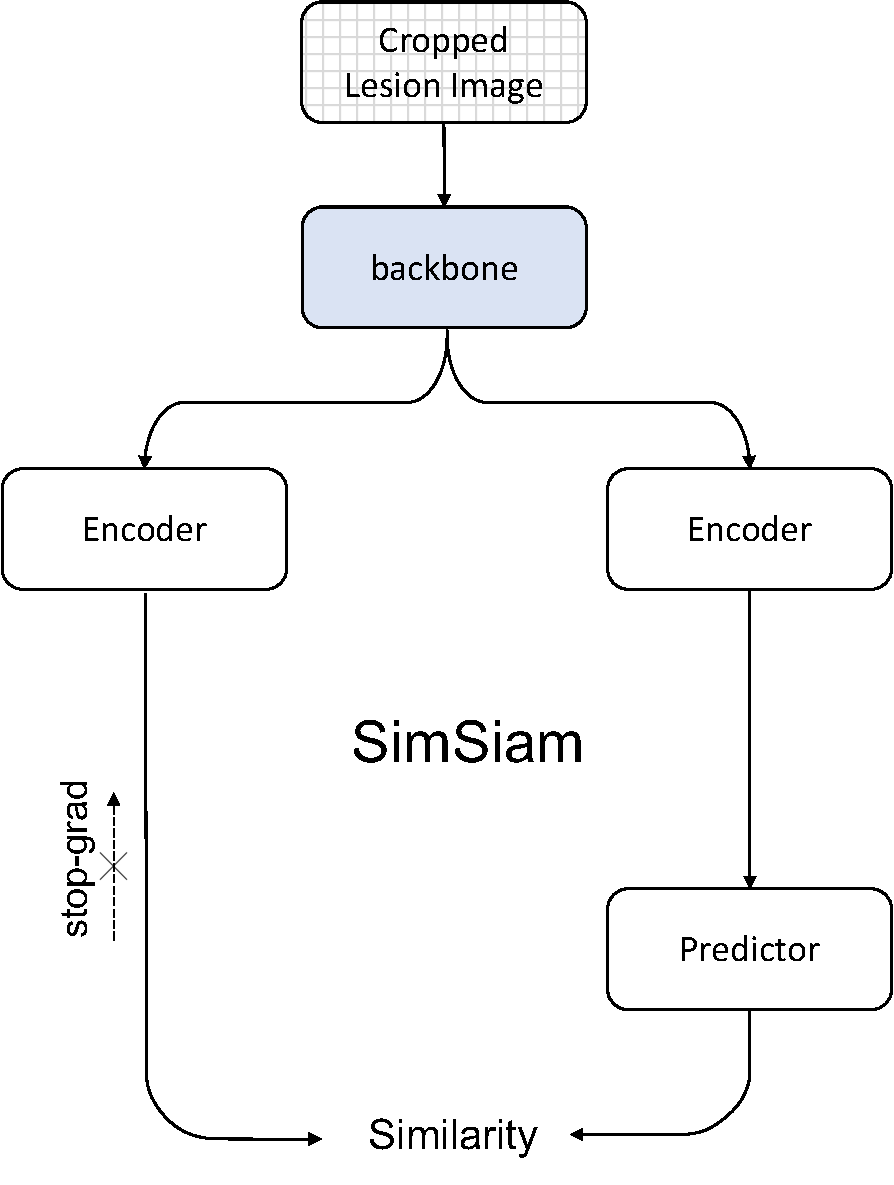
\includegraphics[width=.332\linewidth]{../fig/simsiam.pdf} \label{fig:simsiam}}
            \subfloat[学習及び推論に用いるCenterNet\cite{centernet}の概要]{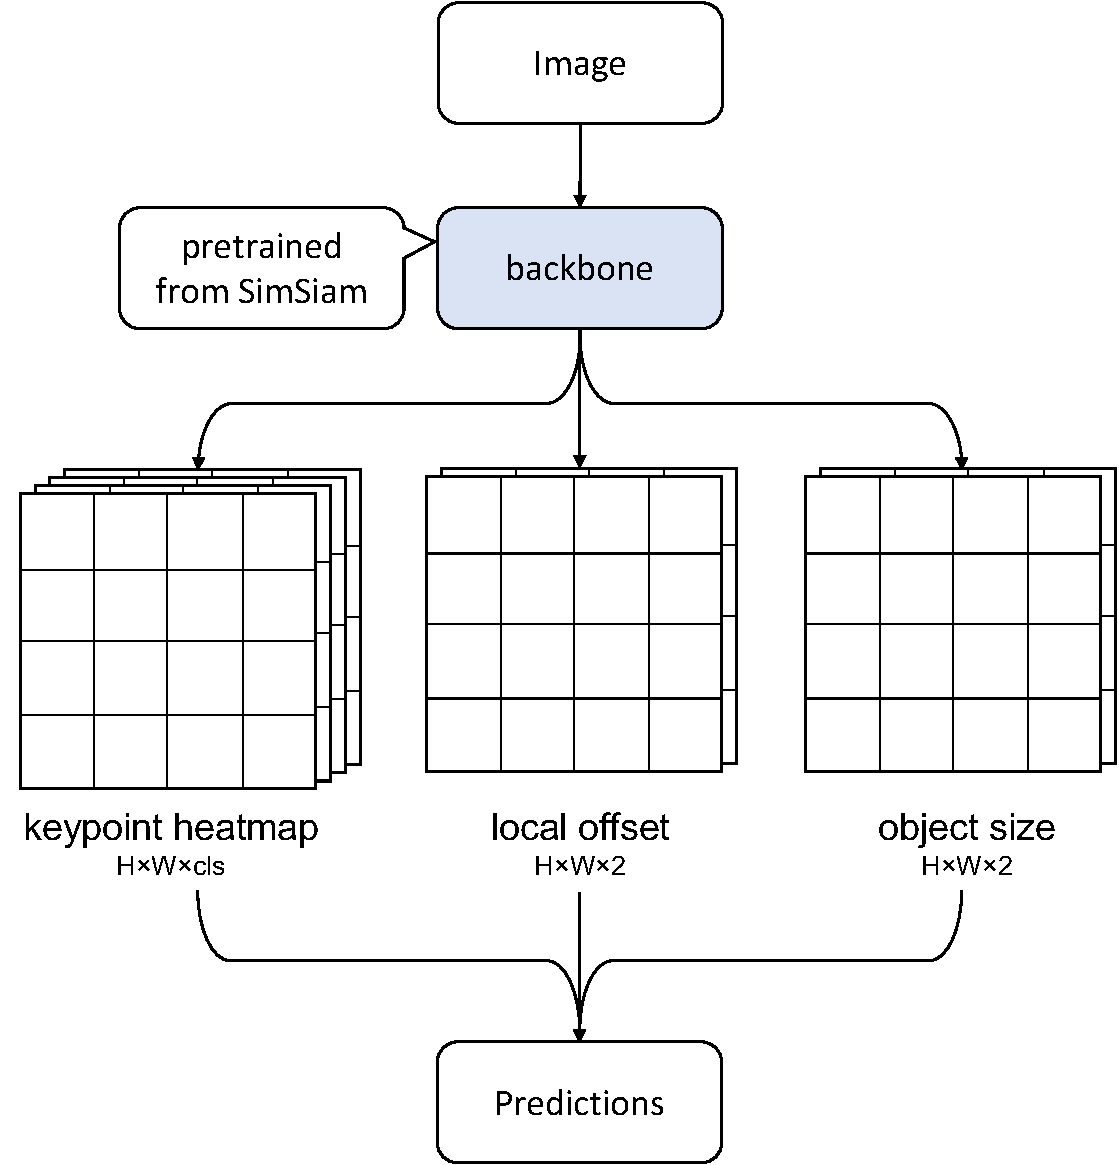
\includegraphics[width=.54\linewidth]{../fig/centernet.pdf} \label{fig:centernet}}
            \caption{4クラス検出の実験で使用したモデル}
        \end{figure}

    \begin{thebibliography}{9}
        \bibitem{yolox} Z. Ge, S. Liu, F. Wang, Z. Li, and J. Sun: ``YOLOX: Exceeding YOLO Series in 2021,'' arXiv preprint, arXiv:2107.08430, 2021.
        \bibitem{simsiam} X. Chen and K. He: ``Exploring simple siamese representation learning,'' Proc. 2021 IEEE/CVF Conf. on Computer Vision and Pattern Recognition, 15750--15758, 2021.
        \bibitem{centernet} X. Zhou et al.: ``Objects as Points,'' arXiv preprint, arXiv:1904.07850, 2019.
        \bibitem{double_descent} Nakkiran, Preetum and Kaplun, Gal and Bansal, Yamini and Yang, Tristan and Barak, Boaz and Sutskever, Ilya: ``Deep double descent: Where bigger models and more data hurt'' Journal of Statistical Mechanics: Theory and Experiment, 124003, 2020.
    \end{thebibliography}
\end{document}
